\section{Statistical Model Checking}

This section will present the UPPAAL SMC extension, the changes to the model made in UPPAAL to utilise this, and also present the results of the queries which are made using the UPPAAL SMC extension.

When a model rely on stochastic behaviors, such as randomness, its state-space grows exponentially (sometimes called a state-space explosion) therefore an exhaustive search determining wheather if some property holds is not possible in reasonable time. 
Instead one can estimate a percentage chance a property holds, within a given probability of uncertainty, with an statistical model checker (SMC). 

%UPPAAL SMC Explanation
\subsection{UPPAAL SMC}
\begin{wrapfigure}[16]{r}{0.3\textwidth}
\centering
  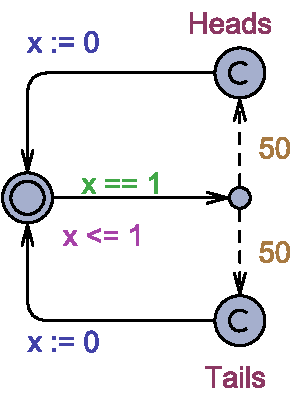
\includegraphics[width=0.3\textwidth]{Figures/Model/Simple_SMC.pdf} 
\caption{A simple UPPAAL SMC model with weighted edges. }
\label{fig:simpleSMC}
\end{wrapfigure}

To do this in UPPAAL there is an extension called UPPAAL SMC, a full tutorial is available here ``Uppaal SMC Tutorial''\cite{DBLP:journals/sttt/DavidLLMP15} by Alexandre David, Kim G. Larsen, Axel Legay, Marius Miku\v{c}ionis, Danny B\o gsted Poulsen.

In UPPAAL SMC there is a new type of edge, this is a weighted edge and is shown as a dashed line. 
An example of this can be seen in figure \myref{fig:simpleSMC}. 
In the figure is a simple UPPAAL SMC model, following the initial state there is a ``branch point'' from which there are two weighted edges.
The number by the weighted edges give their probability of being taken, this simple concept allows UPPAAL SMC to do randomness without having to explore the full state-space, as it can run simulations taking each edge a number of time corresponding to their weights. 
This example simulates a coin toss, giving 50 \% chance of heads and 50 \% chance of tails. 

UPPAAL SMC can additionally draw several types of plots which shows what the chance of a given query being true after a given run duration.

It is possible to set the statistical parameters for UPPAAL SMC, such as: Probability uncertainty, Probability of false negatives and Probability of false positives. 
Setting these parameters closer to zero will cause the time it takes verify a query for a model, however it will also be more accurate. 

%Description of changes to the model in UPPAAL

\subsection*{Changes to the model}

The UPPAAL model shown in \myref{sec:themodel} has gone through extensive changes to accomodate the challenges posed of multiple devices starting at the same time.
The complete model can be seen i the back of the project folder printed on a A3-paper, and it can also be found on the CD, which is also in the back of the project folder.
Since multiple devices are turned on at the same time, it is now possible that more than one device is transmitting at the same time. 
When this happens, it has been mentioned in \myref{subsubsec:RadioHead}, that nothing is detected by the receivers, therefore a mechanism making sure that when two devices are trying to transmit at the same time, nothing will be received by anyone.

The devices can now start at the same time again, as was possible before the mechanism controlling when a device was released was implemented, as presented in \myref{sec:verifyingTheModel}.
To stop devices from being alone in a network forever, a split node is made when nothing is received in a time slot, where the device is alone in the network, i.e. the \texttt{local\_n} of the device is equal to 2.
This split node has 2 outgoing edges, one edge which has a probability weight of 90, which makes the device go back into its main loop, and another edge with a probability of 10, which make the device kill the network, and start listening again.
When this happens the exponential back-off method is used, which means for each time a device kills the network it will have a chance of listening for a longer period of time, according to the specification in the previous sections.
This are the changes needed for the model, in order for the devices to start trying to connect to the same network instead of multiple networks.
The other problem is for when devices try to connect to the same network at the same time.
A verification loop has been created for the model, where all devices which transmitted that they wanted to join the network will listen for the number of devices acknowledging their request of joining the network.
If the amount of acknowledgments are lower than half of the devices in the network, they will also use the exponential backoff method, where they will wait for a random number of frames, in an increasingly larger range, with a cap of 31 frames (It only require one acknowledgment in the CCRC, but this solutions is chosen, to easier expand to CCUC).
This is the only change needed for handling multiple devices connecting to the network, the specifics of the implementation of this on the model will not be presented in this section, but for the curious reader the specifics can be seen in the back as previously mentioned.\todo[inline]{Hvad gør vi med koden der også hører til modellen?} \todo[inline]{Skal der måske alligevel være nogle screenshots af de forskellige dele her ? Det bliver lidt tørt at læse allerede nu synes jeg? Eller er det kun mig der har det sådan ? :) - Søren}

%New Queries using SMC

\subsection*{Verifying using SMC}

Some of the queries presented in \myref{sec:verifyingTheModel} make no sense for this model, as now multiple networks should be running at the same time, and therefore checking if the value of \texttt{i} is the same for all devices in a certain state makes no sense.
It is also of interest to get the probability of the queries being true, rather than checking for true or false.
Therefore the queries will all except for one be checking for the probability of them being true over time, when at least 3000 UPPAAL time units has passed.
It should be noted that the model uses time estimates which roughly translate to the time being used in each phase for the hardware used in this project, where a time-slot is equal to \texttt{Delta} which is set to 250 for this model.

All the queries have been run with five devices in the system, and a confidence of 0.999.
The first query is the only query which was also used on the earlier model, and it will still give a result indicating the query holds.

\begin{lstlisting}[style=UPPAAL, title={This query requires that eventually if all devices are connected, then no pair of devices have the same \texttt{k}, unless the pair consists of the same two devices.}]
1. A<> forall(i : id_t) forall(j : id_t) Device(i).Connected and
         Device(j).Connected and Device(i).k == Device(j).k imply i == j
\end{lstlisting}


\begin{lstlisting}[style=UPPAAL, title={This query asks after 3000 UPPAAL time units has passed, what then is the probability that if two devices \texttt{i}, and \texttt{j} are connected to a network that  their local values of \texttt{n} are the same, and that they are both larger than 2. The query will keep checking the probability until it has been found to be 100\% certain or until 300000 UPPAAL time units has passed.}]
2. Pr[<=300000] ( <> forall(i : id_t) forall(j : id_t)  (time > 3000) 
	  	and (Device(i).Connected and Device(j).Connected imply 
	  	  (Device(i).local_n == Device(j).local_n 
	  		and Device(i).local_n > 2 and Device(j).local_n >2)))
\end{lstlisting}
\noindent
UPPAAL responds with [0.998,1], it is possible to get the data UPPAAL uses to make a graph of the development of the probability over time, which can be seen on \myref{fig:ConnectQueryTime}.


\begin{lstlisting}[style=UPPAAL, title={This query asks after 3000 UPPAAL time units has passed, what then is the probability that a device \texttt{i} has a value \texttt{k} which is different from a device \texttt{j}s value of \texttt{n}}]
3. Pr[<=300000] ( <> forall(i : id_t) forall(j :id_t)  (time >3000) 
		and (Device(i).k != Device(j).local_n))
\end{lstlisting}
UPPAAL will again respond with [0.998,1], but this query just like the next query will actually always be true, and as such cannot be found on the graph, as they are just straight lines.

\begin{lstlisting}[style=UPPAAL, title={This query asks after 3000 UPPAAL time units has passed, what then is the probability that if a device \texttt{i} and a device \texttt{j} is both connected that then \texttt{i}'s values of \texttt{k} will be larger than zero and smaller than \texttt{n}}]
4. Pr[<=300000] ( <> forall(i : id_t) forall(j : id_t)  (time >3000) 
	  and (Device(i).Connected and Device(j).Connected 
	  	imply Device(i).k < Device(i).local_n and Device(i).k > 0))
\end{lstlisting}


\begin{lstlisting}[style=UPPAAL, title={This query asks after 3000 UPPAAL time units has passed, what then is the probability that a device \texttt{i} has a local value of \texttt{n} to be equal to the number of devices, which is \texttt{N} + 1, which means that all devices are in the same network.}]
5. Pr[<=300000] Pr[<=300000] ( <>  forall(i: id_t) (time >3000) 
	and  Device(i).local_n == N+1)
\end{lstlisting}

\noindent This query will also result in [0.998,1] chance, and the development of the probability over time can be seen on \myref{fig:ConnectQueryTime}.

%GRAPHS

\begin{figure}
  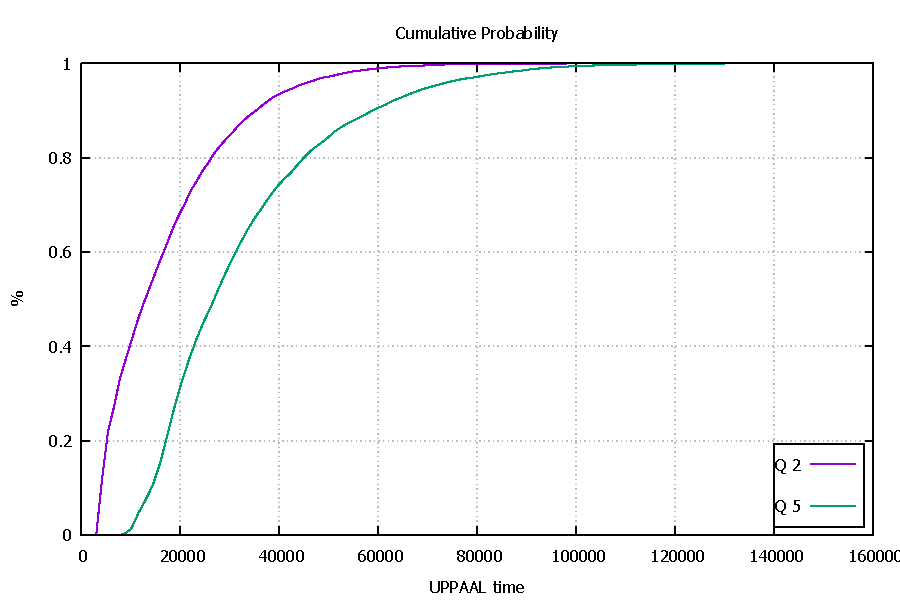
\includegraphics[width=1\textwidth]{Figures/Graphs/ConnectTime.pdf} 
\caption{Graph showing how the probability of the queries 1, and 4 increase over time.}
\label{fig:ConnectQueryTime}
\end{figure}

As can be seen the change in probability increases logarithmically, and will according to UPPAAL eventually connect, however it might take some time for it to do so.
This is because in the worst case the random numbers generated will keep causing collisions, or maybe they will take a long time before eventually killing their networks.
There are many possible explanations for what causes the longer runs, but it it important to note the fact that, the longer the devices are running the bigger the chances are of establishing a stable network.

\todo[inline]{Ide: Måske kunne vi vise hvorfor nogle runs tager lang tid: ``Anatomy of a slow run''. Så kan vi vise hvad der skal ske for at det går dårligt. }

%Conlusion

\section{Conclusion}
This chapter presented a way to handle the startup of multiple devices, which made use of the technique exponential back-off, which results in an increasingly randomly generated number of wait time for the devices. 
The randomness results in all devices eventually becoming connected to the network since they will be split up and thus stop jamming each other.
The UPPAAL model created data, which can be seen on \myref{fig:ConnectQueryTime}.
The data shows that the Arduinos will eventually be connected to the same network, however it does take some time, approximately 150k UPPAAL time units.
This means that an implementation of this design should theoretically be able to solve the issues of turning on more Arduinos at the same time.
